\documentclass{article}
\usepackage{graphicx}
\usepackage{wrapfig}
\usepackage{xcolor}
\usepackage{hyperref}
\usepackage{multicol}

\setlength{\textheight}{25cm}
\setlength{\textwidth}{152mm}
\setlength{\topmargin}{-2.5cm}
\setlength{\evensidemargin}{12mm}
\setlength{\oddsidemargin}{6mm}
\definecolor{my_col}{RGB}{0,150,150}
\pagenumbering{gobble}

\sffamily

\begin{document}

\begin{center}
	\textit{\Huge Curriculum Vitae}   
	\vspace*{1cm}
\end{center}

\begin{wrapfigure}{r}{0.25\textwidth} 
	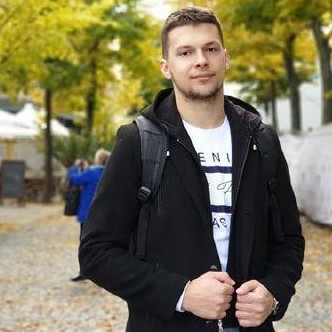
\includegraphics[width=0.25\textwidth]{my_pic.jpeg}
\end{wrapfigure}

\color{my_col}
\textbf{\large PERSONAL INFORMATION}\\
\noindent\rule{10cm}{1.5pt}\color{black}\\ \\
Name:  \textbf{\emph{Predrag MITIC}} \\
Address: \emph{Bulevar Zorana Djindjica, Belgrade, Serbia }\\
Tel: 	(+381) 61 18 56 816 \\
E-mail1:	\textit{predrag98mitic@gmail.com} \\ 
E-mail2:	\textit{pmitic@hotmail.com} \\ 
Web:	\url{www.alas.matf.bg.ac.rs/~mi17116} \\
Github:	\url{www.github.com/PredragMitic} \\ 
LinkedIn: \url{www.linkedin.com/in/predrag-mitic-353019188}\\
Date of Birth: September 1, 1998 \\ 

\color{my_col}
\textbf{\large PROFILE}\\
\noindent\rule{15.4cm}{1.6pt}\color{black}\\ 
Ambitious and highly motivated third year student at Faculty of Mathematics, 
University of Belgrade. With practical experience in Computer Graphics and 
C/C++ programming languages. Team player, quick learner, open to new ideas and experiences.\\ \\
\textit{\textbf{English level: } B1+}\\

\color{my_col}
\textbf{\large PROGRAMMING LANGUAGES}\\
\noindent\rule{15.4cm}{1.6pt}\color{black}
\normalsize
\begin{itemize}
	\item\textbf{Good knowledge: 	} C/C++, Python3, Java
	\item\textbf{Some experience:	} Haskell, Scala, R, JavaScript
	\item\textbf{Frameworks used:} JavaFX, QT5\\
\end{itemize}
  
\color{my_col}
\textbf{\large COMPUTER SKILLS}\\
\noindent\rule{15.4cm}{1.6pt}\color{black}
\normalsize
   \begin{multicols}{2}
  	\begin{itemize}
  		\item\textbf{OS: 	} Windows, GNU/Linux
  		\item\textbf{Documents:} MS Office, Libre Office, \LaTeX
  		\item\textbf{Markup Language: } HTML, CSS\\
  		\item\textbf{Image editing: } Gimp
  		\item\textbf{Editors :} Vim, JetBrains(CLion, PyCharm, Idea),
  		Visual Studio (Code), Jupyter Notebook, Atom, Emacs\\
 
  	\end{itemize}
  \end{multicols}

\color{my_col}
\textbf{\large EMPLOYMENTS AND TRAINING}\\
\noindent\rule{15.4cm}{1.6pt}\color{black}
\begin{description}
	\item[ 2019] - RT-RK Summer School \\
	\textit{Modern Improvements in C++}\\
\end{description}

\color{my_col}
\textbf{\large PROJECTS}\\
\noindent\rule{15.4cm}{1.6pt}\color{black}
\begin{description}
	\item[ C/OpenGL] - Shoot Training\\ 
	Game made in C program language and OpenGl(Open Graphics Library)
	\item[ HTML/NodeJS] - Web Library\\ 
	Web page for online book library powered by NodeJS
	\item[ Python3/Pygame] - Star Wars Space Battle\\ 
	Game like Galaga made in pygame with Star Wars motives.\\
	This game is built by team Jedi-MATF for course project.
\end{description}
My projects with other details can be seen on my GitHub profile \\

\color{my_col}
\textbf{\large SCIENTIFIC INTERESTS}\\
\noindent\rule{15.4cm}{1.6pt}\color{black}\\\\
- Algorithm and Data Structures\\
- Data science \\
- Computer Graphics and Game Development\\
- Mobile App Development\\

\color{my_col}
\textbf{\large EDUCATION}\\
\noindent\rule{15.4cm}{1.6pt}\color{black}
\begin{description}
    \item[ 2017-present : Bachelor of Informatics ]\hfill \\
    \textbf{\textit{Faculty of Mathematics, University of Belgrade}}\\
    \normalsize \\
    Subjects studied :
     \begin{multicols}{2}
    \begin{itemize}
    \item Programming
    \item Computer Architecture
    \item Algorithms and Data structures
    \item Operating Systems
    \item Database Systems
    \item Web programming
    \item Geometry
    \item Numerical Mathematics
    \item Probability and Statistics 
    \item English
    \end{itemize}
    \end{multicols}
\end{description}

\begin{description}
    \item[ 2013-2017 : Mechatronics Technician]\hfill \\
    \textbf{\textit{High School of Technology, Leskovac}}\\
    \normalsize \\
  
\end{description}
\color{my_col}
\textbf{\large ACHIEVEMENTS}\\
\noindent\rule{15.4cm}{1.6pt}\color{black}
\normalsize

\begin{description}
	\item[ 2016] - Fourth place in 3D Computer Graphics (Autodesk Inventor)\\
	National Competition
	\item[ 2016] - Second place in Electronics\\
	National Competition
	\item[ 2015] - First place in 2D Computer Graphics (Autodesk AutoCAD)\\
	Regional Competition
	\item[ 2014] - First place in 2D Computer Graphics (Autodesk AutoCAD)\\
	National Competition
\end{description}

\color{my_col}
\textbf{\large FREE TIME }\\
\noindent\rule{15.4cm}{1.6pt}\color{black}\\\\
- Travel and Languages\\
- Sport (Basketball, Football, Tennis) \\
- Art (Movies, Music, Books)\\
- Geography\\

\color{my_col}\noindent\rule{15.4cm}{1.6pt}\color{black}
\begin{flushright}
	\small Belgrade, June 4, 2020
\end{flushright}

\end{document}